\documentclass[tikz,border=3pt]{standalone}
\usepackage[utf8]{inputenc}
\usepackage{pgfplots}
\usepgfplotslibrary{groupplots}
\pgfplotsset{compat=1.18}

\definecolor{timeoutgray}{HTML}{5F6B76}
\definecolor{unsatorange}{HTML}{D55E00}

\begin{document}
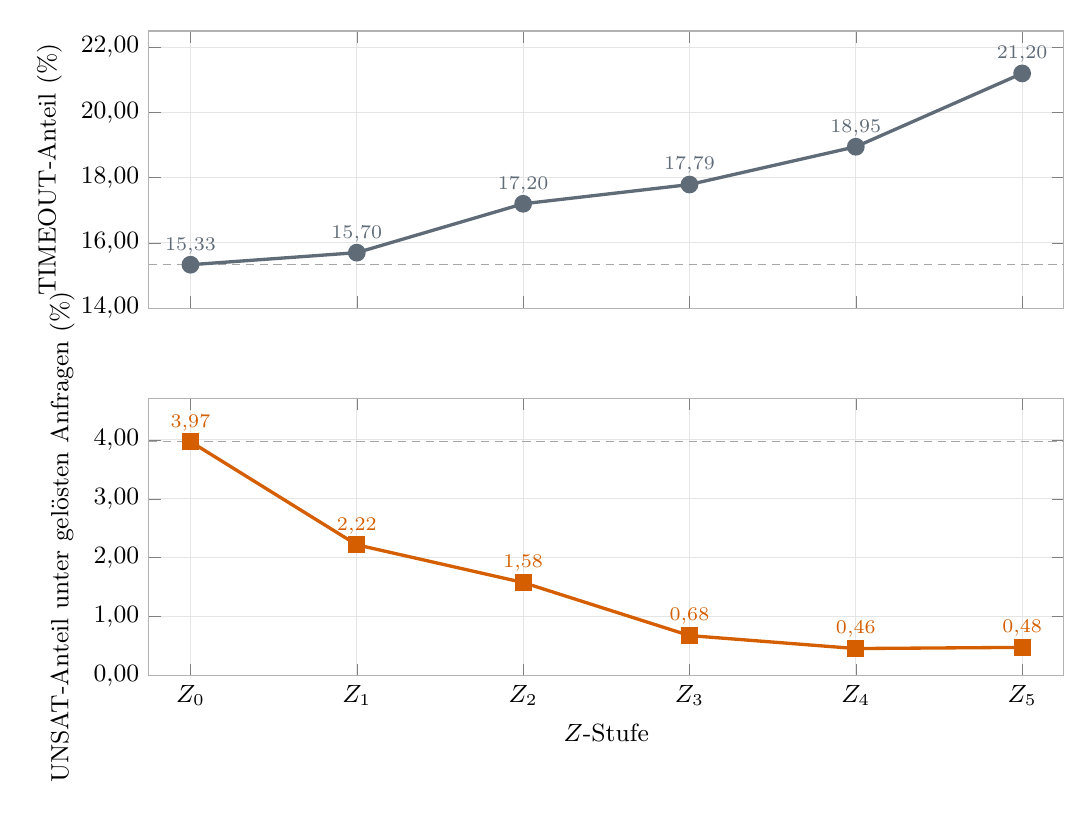
\begin{tikzpicture}
\begin{groupplot}[
    group style={group size=1 by 2,vertical sep=1.15cm},
    width=13.2cm,
    height=5.1cm,
    xmin=-0.25,
    xmax=5.25,
    xtick={0,1,2,3,4,5},
    xticklabels={$Z_0$,$Z_1$,$Z_2$,$Z_3$,$Z_4$,$Z_5$},
    grid=major,
    grid style={draw=gray!20},
    axis line style={draw=gray!60},
    tick label style={font=\small},
    label style={font=\small},
    /pgf/number format/fixed,
    /pgf/number format/fixed zerofill,
    /pgf/number format/precision=2,
    /pgf/number format/use comma
]
\nextgroupplot[
    ymin=14,
    ymax=22.5,
    ytick={14,16,18,20,22},
    ylabel={TIMEOUT-Anteil (\%)},
    xticklabels={}
]
\addplot+[densely dashed,draw=gray!70,forget plot,no marks]
    coordinates {(-0.25,15.33) (5.25,15.33)};
\addplot+[
    very thick,
    mark=*,
    mark size=2.6pt,
    draw=timeoutgray,
    fill=none,
    mark options={fill=timeoutgray},
    nodes near coords,
    every node near coord/.append style={
        font=\scriptsize,anchor=south,text=timeoutgray
    },
    point meta=y
]
    coordinates {(0,15.33) (1,15.70) (2,17.20) (3,17.79) (4,18.95) (5,21.20)};

\nextgroupplot[
    ymin=0,
    ymax=4.7,
    ytick={0,1,2,3,4},
    ylabel={UNSAT-Anteil unter gelösten Anfragen (\%)},
    xlabel={$Z$-Stufe}
]
\addplot+[densely dashed,draw=gray!70,forget plot,no marks]
    coordinates {(-0.25,3.97) (5.25,3.97)};
\addplot+[
    very thick,
    mark=square*,
    mark size=2.5pt,
    draw=unsatorange,
    fill=none,
    mark options={fill=unsatorange},
    nodes near coords,
    every node near coord/.append style={
        font=\scriptsize,anchor=south,text=unsatorange
    },
    point meta=y
]
    coordinates {(0,3.97) (1,2.22) (2,1.58) (3,0.68) (4,0.46) (5,0.48)};
\end{groupplot}
\end{tikzpicture}
\end{document}
